\documentclass[11pt]{article}
\usepackage[a4paper,margin=1in]{geometry}
\usepackage{hyperref}
\usepackage{booktabs}
\usepackage{enumitem}
\usepackage{listings}
\usepackage{xcolor}
\usepackage{tikz}
\usetikzlibrary{positioning,arrows.meta,shapes.geometric}

\lstset{
  basicstyle=\ttfamily\small,
  breaklines=true,
  frame=single
}

\title{\textbf{RiskMapper: Risk and Attack Surface Mapping Tool}\\
\large CVSS-Based Vulnerability Prioritization (Scanning, CVSS, Attack Surface)}
\author{Student Name \quad | \quad CSS Module}
\date{\today}

\begin{document}
\maketitle

\begin{abstract}
RiskMapper is a desktop application built with Python and Flet that converts vulnerability scanning data
(or manual metric input) into a standardized risk assessment using the CVSS v3.1 Base Score. The tool
classifies findings by severity, generates a CVSS vector string, maps vulnerabilities to attack-surface
assets (tags and exposed services), and persists data in SQLite so results remain available across restarts.
\end{abstract}

\section{Objectives}
The project goals are:
\begin{itemize}[leftmargin=*]
  \item Implement CVSS v3.1 Base Score computation from base metrics (AV, AC, PR, UI, S, C, I, A).
  \item Display the final score and its severity class to support remediation prioritization.
  \item Generate a standard CVSS vector string (e.g., \texttt{CVSS:3.1/AV:N/AC:L/...}).
  \item Import multiple findings from CSV/JSON (simplified scan export formats).
  \item Model attack surface through assets (hostname/IP/app), tags, and exposed services/ports.
  \item Provide export to CSV, including a filtered export for selected assets.
  \item Persist assets and findings in SQLite for durability across application restarts.
\end{itemize}

\section{Background: Scanning, CVSS, and Prioritization}
Vulnerability scanners often produce large result sets. Without a prioritization mechanism, remediation
becomes inefficient. CVSS (Common Vulnerability Scoring System) provides a standardized way to rank
vulnerabilities by severity. RiskMapper focuses on the CVSS v3.1 \textbf{Base Score}, which combines:
\begin{itemize}[leftmargin=*]
  \item \textbf{Exploitability}: Attack Vector (AV), Attack Complexity (AC), Privileges Required (PR),
        User Interaction (UI).
  \item \textbf{Impact}: Confidentiality (C), Integrity (I), Availability (A), and Scope (S).
\end{itemize}

\section{System Overview}
\subsection{Technology Choice}
Flet was selected to build a modern GUI in Python with an event-driven model (buttons, tabs, dialogs).
SQLite was selected for lightweight local persistence without requiring a server.

\subsection{High-level Architecture}
RiskMapper is divided into modules:
\begin{itemize}[leftmargin=*]
  \item \texttt{main.py}: Flet GUI with tabs (Dashboard, Calculator, Import, Assets) and user workflows.
  \item \texttt{cvss.py}: CVSS v3.1 Base Score logic, severity mapping, and vector string generation.
  \item \texttt{parser.py}: CSV/JSON parsing into finding records.
  \item \texttt{db.py}: SQLite schema and CRUD operations (assets and findings).
  \item \texttt{storage.py}: In-memory model objects synchronized with SQLite (load on startup, write on change).
  \item \texttt{ui\_components.py}: UI helpers (cards, pills, snackbars).
\end{itemize}

\subsection{Architecture Diagram (Data Flow)}
\begin{center}
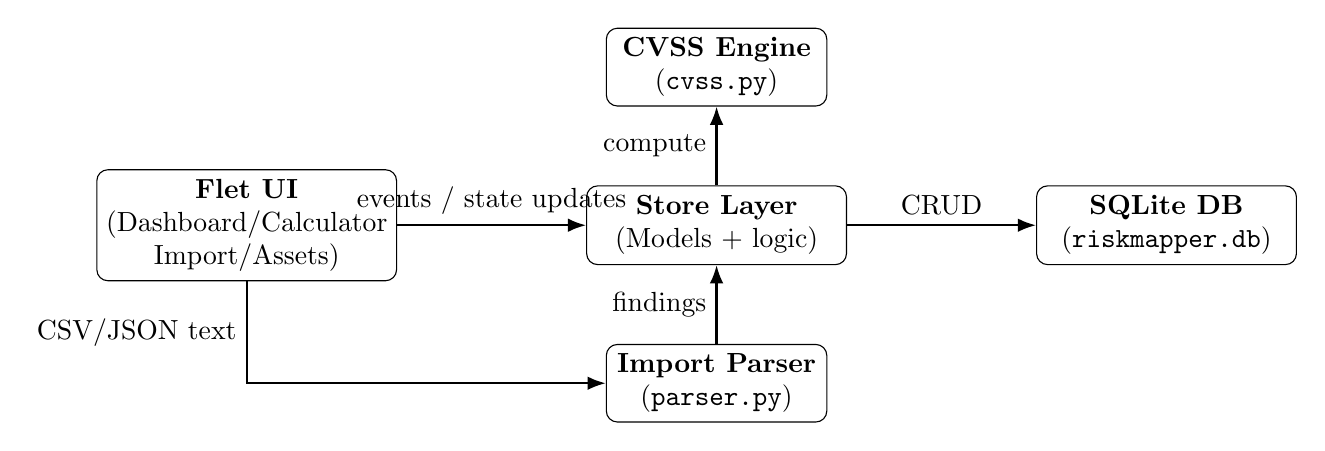
\begin{tikzpicture}[
  node distance=12mm,
  box/.style={draw, rounded corners, align=center, minimum width=3.3cm, minimum height=1.0cm},
  smallbox/.style={draw, rounded corners, align=center, minimum width=2.8cm, minimum height=0.85cm},
  arrow/.style={-Latex, thick}
]
\node[box] (ui) {\textbf{Flet UI}\\(Dashboard/Calculator\\Import/Assets)};
\node[box, right=24mm of ui] (store) {\textbf{Store Layer}\\(Models + logic)};
\node[smallbox, above=10mm of store] (cvss) {\textbf{CVSS Engine}\\(\texttt{cvss.py})};
\node[smallbox, below=10mm of store] (parser) {\textbf{Import Parser}\\(\texttt{parser.py})};
\node[box, right=24mm of store] (sqlite) {\textbf{SQLite DB}\\(\texttt{riskmapper.db})};

\draw[arrow] (ui) -- node[above]{events / state updates} (store);
\draw[arrow] (store) -- node[above]{CRUD} (sqlite);
\draw[arrow] (store) -- node[left]{compute} (cvss);
\draw[arrow] (parser) -- node[left]{findings} (store);
\draw[arrow] (ui) |- node[left, near start]{CSV/JSON text} (parser);

\end{tikzpicture}
\end{center}

\section{CVSS v3.1 Base Score Implementation}
\subsection{Supported Metrics}
\begin{center}
\begin{tabular}{ll}
\toprule
Metric & Values \\
\midrule
AV & N, A, L, P \\
AC & L, H \\
PR & N, L, H (depends on Scope) \\
UI & N, R \\
S  & U, C \\
C/I/A & H, L, N \\
\bottomrule
\end{tabular}
\end{center}

\subsection{Computation Summary}
The CVSS Base Score is computed using:
\begin{itemize}[leftmargin=*]
  \item Exploitability $= 8.22 \times AV \times AC \times PR \times UI$
  \item ImpactSubScore $= 1 - (1-C)(1-I)(1-A)$
  \item Scope affects the impact function and may apply a scaling factor.
  \item Final score is capped at 10.0 and \textbf{rounded up} to one decimal (CVSS requirement).
\end{itemize}

\subsection{Vector String Generation}
RiskMapper generates a standard CVSS v3.1 vector string:
\[
\texttt{CVSS:3.1/AV:N/AC:L/PR:N/UI:R/S:U/C:L/I:L/A:N}
\]
This representation is useful for reporting and interoperability. The vector is displayed in the UI and
stored in the database for each finding (and can be copied to clipboard).

\subsection{Severity Levels}
\begin{itemize}[leftmargin=*]
  \item None: 0.0
  \item Low: 0.1--3.9
  \item Medium: 4.0--6.9
  \item High: 7.0--8.9
  \item Critical: 9.0--10.0
\end{itemize}

\section{Attack Surface Mapping}
Attack surface is represented by \textbf{Assets}:
\begin{itemize}[leftmargin=*]
  \item \textbf{Asset name}: hostname, IP address, or application identifier.
  \item \textbf{Tags}: context (e.g., internet-facing, production, PCI).
  \item \textbf{Services}: exposed ports/protocols (e.g., 443/https, 22/ssh).
\end{itemize}
Findings are linked to assets by matching the asset name (normalized by trimming and case-insensitive comparison).
The Assets tab provides asset-centric risk summaries, enabling quick identification of the riskiest systems.

\section{Data Import and Export}
\subsection{Import Formats}
RiskMapper supports:
\begin{itemize}[leftmargin=*]
  \item CSV header: \texttt{asset,title,AV,AC,PR,UI,S,C,I,A}
  \item JSON list of objects with the same keys.
\end{itemize}
Invalid rows (incorrect metric codes) are skipped for robustness.

\subsection{Export Features}
The application provides:
\begin{itemize}[leftmargin=*]
  \item \textbf{Export all findings to CSV} from the Dashboard.
  \item \textbf{Filtered export}: export findings for \textbf{multiple selected assets} into a single CSV file.
\end{itemize}
Exported CSV includes score, severity, vector string, and the selected metrics.

\section{Persistence with SQLite}
To preserve data across restarts, RiskMapper stores:
\begin{itemize}[leftmargin=*]
  \item Assets in an \texttt{assets} table (name, tags, services).
  \item Findings in a \texttt{findings} table (asset, title, metrics, score, severity, vector).
\end{itemize}
On startup, the app loads all records into memory. When assets or findings are created or deleted, the
SQLite database is updated accordingly.

\subsection{SQLite Schema}
The database is stored locally as \texttt{riskmapper.db}. Two main tables are used:

\begin{center}
\begin{tabular}{lll}
\toprule
\textbf{Table} & \textbf{Column} & \textbf{Description} \\
\midrule
assets & id (PK) & Unique identifier (UUID as text) \\
assets & name (UNIQUE) & Asset name (hostname/IP/app) \\
assets & tags & Comma-separated tags (internet-facing, prod, ...) \\
assets & services & Comma-separated services (443/https, 22/ssh, ...) \\
assets & created\_at & Insert timestamp \\
\midrule
findings & id (PK) & Unique identifier (UUID as text) \\
findings & asset\_name & Asset name linked to findings \\
findings & title & Finding title/short description \\
findings & av,ac,pr,ui,s,c,i,a & CVSS base metrics (stored as codes) \\
findings & score & CVSS base score (REAL) \\
findings & severity & Severity label (None/Low/Medium/High/Critical) \\
findings & vector & CVSS vector string \\
findings & created\_at & Insert timestamp \\
\bottomrule
\end{tabular}
\end{center}

An index is created on \texttt{findings(asset\_name)} to accelerate asset-centric queries.

\section{Functional Requirements}
\begin{itemize}[leftmargin=*]
  \item FR1: Compute CVSS v3.1 Base Score from user-selected base metrics.
  \item FR2: Display score, severity, and vector string for each finding.
  \item FR3: Import findings from CSV/JSON and compute scores in bulk.
  \item FR4: Create and manage assets (tags and exposed services).
  \item FR5: Persist assets and findings in SQLite across restarts.
  \item FR6: Export findings to CSV (global and selected assets).
  \item FR7: Allow multi-selection of assets and toggle selection (click again to deselect).
\end{itemize}

\section{Non-Functional Requirements}
\begin{itemize}[leftmargin=*]
  \item NFR1: Usable GUI with clear navigation (tabs) and feedback messages.
  \item NFR2: Robust validation: invalid metric codes are rejected (calculator) or skipped (import).
  \item NFR3: Lightweight local storage (SQLite), no external services required.
  \item NFR4: Maintainable code structure with separated modules (UI, CVSS logic, persistence).
\end{itemize}

\section{User Stories / Use Cases}
\begin{center}
\begin{tabular}{p{2.8cm}p{10.8cm}}
\toprule
\textbf{Actor} & \textbf{User story / Use case} \\
\midrule
Student / Analyst & As a user, I want to calculate a CVSS v3.1 Base Score by selecting the base metrics, so that I can classify the vulnerability severity. \\
\midrule
Student / Analyst & As a user, I want to save a finding (asset, title, metrics, score, severity, vector) so that it persists and can be reviewed later. \\
\midrule
Student / Analyst & As a user, I want to import multiple findings from CSV/JSON so that I can quickly score scan outputs in bulk. \\
\midrule
Student / Analyst & As a user, I want to manage an asset inventory (tags, exposed services) so that I can represent the attack surface. \\
\midrule
Student / Analyst & As a user, I want to view risk per asset (max/avg score, severity counts) so that I can prioritize remediation on the most exposed/high-risk systems. \\
\midrule
Student / Analyst & As a user, I want to generate and copy the CVSS vector string so that I can include it in reports and tickets. \\
\midrule
Student / Analyst & As a user, I want to export findings to CSV (all findings or selected assets) so that I can submit a report or share results. \\
\bottomrule
\end{tabular}
\end{center}

\section{User Interface (Tabs)}
\begin{itemize}[leftmargin=*]
  \item \textbf{Dashboard}: severity counters, latest findings, and global CSV export.
  \item \textbf{Calculator}: CVSS metric selection, score/severity result, vector display/copy, save to DB.
  \item \textbf{Import}: paste/load CSV or JSON, bulk scoring, skip invalid rows, store results.
  \item \textbf{Assets}: create assets, multi-select assets (toggle), last-selected details, filtered CSV export, delete.
\end{itemize}

\section{Conclusion and Future Work}
RiskMapper demonstrates an end-to-end workflow from vulnerability metrics to actionable prioritization:
CVSS scoring, standardized vectors, and attack surface mapping with asset-centric analytics. SQLite persistence
makes the tool practical for repeated use. Future enhancements may include role-based access, richer scan imports
(Nmap XML, Nessus), trend dashboards, and SLA tracking.

\end{document}
